\chapter{Related Work}
This chapter presents the related work on which this project will be built on. The basis will be the work done at General Acoustics e.K. particularly from Dipl. Ing. Jan Schirrmacher in previous projects containing an ADCP. Afterwards an in-depth introduction on the used ADCP from Rowe Technologies, Inc. will provide the needed background information. Finally the used external libraries will be presented to give background information needed further in the report.

\section{General Acoustics e.K.}
Due to previous projects with ADCP's a lot of knowledge about the technology was allready available from General Acoustics e.K. A look at the algorithms of the current ADCP parser as well as other libraries used in this context gave a goot introduction into the problems and helped a lot in architectural decisions. The libraries were developed by Jan Schirrmacher in Delphi and thus only available for Windows.

\section{Acoustic Doppler Current Profiler}
An Acoustic Doppler Current Profiler (ADCP) is a hydro-acoustic instrument or sonar device that is used to measure water velocities in discrete layers over a certain range that is defined by the acoustic frequency. Essentially, the ADCP emits a sound signal of a specific frequency and measures the return frequency that is received from backscatter via particles in the water column [1].

The reference ADCP used for this project is produced by Rowe Technologies [2]. It has 4 horizontal pistons and one vertical piston, also known as beams. Beams emit the waves used to measure the flow currents and directions.\\
\begin{figure}[h]
\centering
      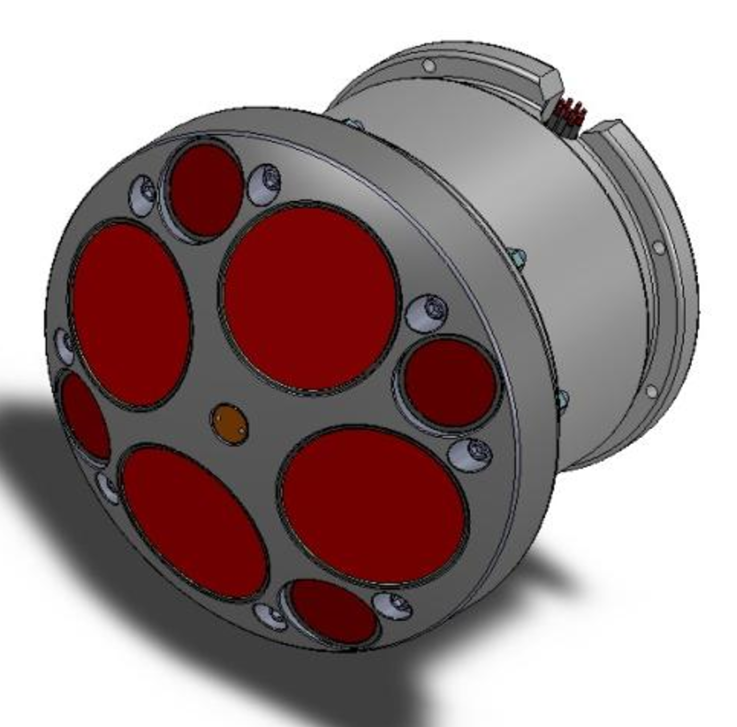
\includegraphics[width=0.8\textwidth]{adcp}
        \caption{A picture of the ADCP referenced in this project. }
\end{figure}
The used ADCP is configured to measure a maximum of 15 meter distance devided into 30 discreet bins of 0.5m. The 4 horizontal beams are used to measure the flow currents and directions, internal signal processing is used to calculate the correct earth coordinates (East, North, Up) based on an the ADCP position and Heading, Pitch and Roll angles. The single beam is used to measure the water level.\\
The ADCP is configured to ping at 6Hz always alternating eighter horizontal or vertical ping. It operates in bursts, one burst every 10 minutes. One burst consists of 2048 pings where 1024 are horizontal and 1024 are vertical pings. A ping is also called ensemble. Therefore a burst is defined as a collection of 2048 ensembles, measured over a period of ~6-7 minutes. An ensemble contains the data of one ping, the structure of the data is presented furtheron in the report. The collected data is then sendt burstwise over RS485 at 460800 Baud to a datalogger on the offshore platform.

An ADCP ensemble consists of three sections. The first section is a 32 byte header. The header consists of 16 bytes containing 0x80, followed by a four byte uint32 ensemble number. The next four bytes contain the ones-compliment of the ensemble number. The last eight bytes contain the uint32 payload size in bytes as well as its ones-compliment.\\
The middle section contains the payload as Matlab version 4 file. A Matlab-file may contain one or more matrices. The matrices are written sequentially to a file, with the bytes forming a continuous stream. Each matrix starts with a fixed-length 20-byte header that contains information describing certain attributes of the Matrix. The 20-byte header consists of five long 4-byte integers. After the Header the matrix data follows in the numerical fromat specified in the header. The data contains rows $\cdot$ columns elements.
The payload of an ensemble contains a series of matrices named E000001 to E000015. Depending on the ensemble type not all matrices may be available.\\
The last part is a four byte CRC16 checksum over all bytes in the payload. The first two bytes are always 0, the second two bytes contain the CRC16 value. The value is based on the CCITT 16 bit algorithm following the formula 

$$ x^{16} + x^{12} + x^5 +1$$

with CRC seed of value 0.

If the 32 byte header is removed from each ensemble, Matlab is able to read in the ensembles.
\begin{figure}[h]
\centering
      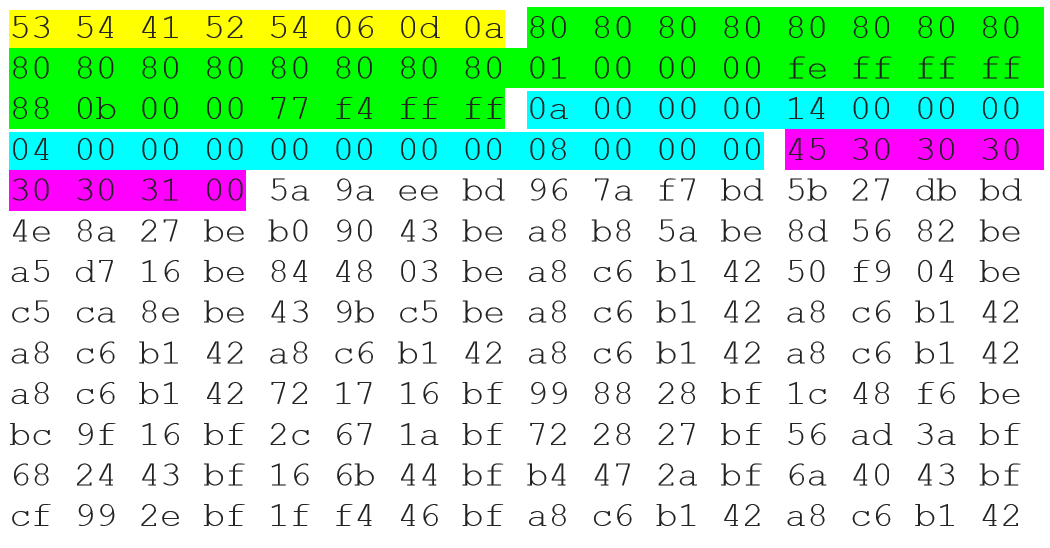
\includegraphics[width=0.8\textwidth]{hexdump}
        \caption{A hex-capture of the first few bytes from an ensemble- }
\end{figure}

Figure 2.2 shows the first few bytes of an ensemble.
\begin{itemize}
\item Yellow marked is the word START followed by CRLF. This was captured when the ADCP was started.
\item Green colored is the 32 byte ensemble header, it begins with the 16 bytes of 0x80.
\item  Cyan is the matlab version 4 matrix-header containing 4 integer values are that are set to 10,20,4, and 8.  
\begin{itemize}
\item The 10 indicates the matrix contains 4 byte floating point numbers. 
\item 20 is the number of rows in the matrix which is number bins in the ADCP profile. 
\item 4 is the number of columns which is the number of ADCP profile beams.  
\item 8 is the number of bytes in the matrix name.  
\end{itemize}
\item Pink is the matrix name ``E000001''
\item Following that Following that there is 4*20 = 80 floating point numbers in the matrix (not all shown here).
\item The next matrix ``E000002'' starts after the last floating point number... and so on until all of the matrices in the ensemble are read in
\item The end of the ensemble has 4 more bytes that are used as a checksum. 
\item The next ensemble starts with a 32 byte header just like the previous one and contains the same matrix names repeated but with new data. 
\end{itemize}

The present the content of all 15 matrices would go beyond the scope of this report, thus only the important matrices are described. The other matrices contain additional information e.g. ping quality, and are thrown away in the parsing process in developed software to reduce the size of the logged files.\\

The matrices that are used for further processing are:
\begin{itemize}
\item ``E000001'' - Bins $\times$ Beams of single precision floating points containing  the Beam coordinate velocity profile data as measured along each beam. The data is useful for diagnostic purposes and for when the user wants to perform their own transformation. In the context of this project the data is only used for further wave analysis, and only from the vertical pings.
\item``E000003'' - Bins $\times$ Beams of single precision floating points containing the Earth coordinate velocity profile in m/s. 
\item ``E000008'' - Twentytwo 32 bit Integers containing various ensemble data, the ensemble number, timestamp, number of bins and beams as well as the ADCP system configuration.
\item ``E000009'' - Thirteen single precision floating points containing various ancillary data, e.g. water pressure and water temperature.
\item ``E000015'' - 1 + 3 $\times$ Beams of single precision floating points containing e.g. the water level. 
\end{itemize}

\section{Libraries}
For the implementation of this project, a number of external libraries were used to simply the developement process. The decision for or against various libraries is illustrated in Chapter 3, at this point, only the libraries used in the implementation are described.
\subsection{Boost}
Boost is a collection of libraries
\subsection{Lockfree Queues}

\subsection{Serial Port Wraper}